\documentclass [xcolor=svgnames, t] {beamer} 
\usepackage[utf8]{inputenc}
\usepackage{booktabs, comment} 
\usepackage[absolute, overlay]{textpos} 
\useoutertheme{infolines} 
\setbeamercolor{title in head/foot}{bg=internationalorange}
\setbeamercolor{author in head/foot}{bg=dodgerblue}
\usepackage{csquotes}
\usepackage[style=verbose-ibid,backend=bibtex]{biblatex}
\bibliography{bibfile}
\usepackage{fontawesome}
\usepackage{amsmath}



\usepackage{textpos}



\usetheme{Madrid}
\definecolor{myuniversity}{RGB}{0, 60, 113}
\definecolor{internationalorange}{RGB}{231, 93,  42}
 	\definecolor{dodgerblue}{RGB}{0, 119,202}
\usecolortheme[named=myuniversity]{structure}
\usepackage{tikz}



\title[Project Logistic Module]{Project Logistic Module}
\subtitle{Software Development}
\titlegraphic{\hfill\includegraphics[height=1.5cm]{Logo_université_montpellier.png}}
\author[C. Delage, H. Bacave, Y. Mimouni]{{Hanna Bacave, Yassine Mimouni, Cindy Delage } \\
\faGithub\href{https://github.com/hannabacave/logistic_module}{ Logistic module} }

\institute[]{Masters MIND-Biostatistic, Montpellier University}



\date{May 25, 2020}


\addtobeamertemplate{navigation symbols}{}{%
    \usebeamerfont{footline}%
    \usebeamercolor[fg]{footline}%
    \hspace{1em}%
    \insertframenumber/\inserttotalframenumber
}

\begin{document}


\begin{frame}
 \titlepage   
\end{frame}

\begin{frame}{Table Of Contents}
\tableofcontents
\end{frame}


\begin{frame}
\frametitle{Introduction}
\section{Introduction}
    \begin{figure}[!h]
    \begin{center}
   \caption{\label{étiquette} Survey results on 85 individuals}
   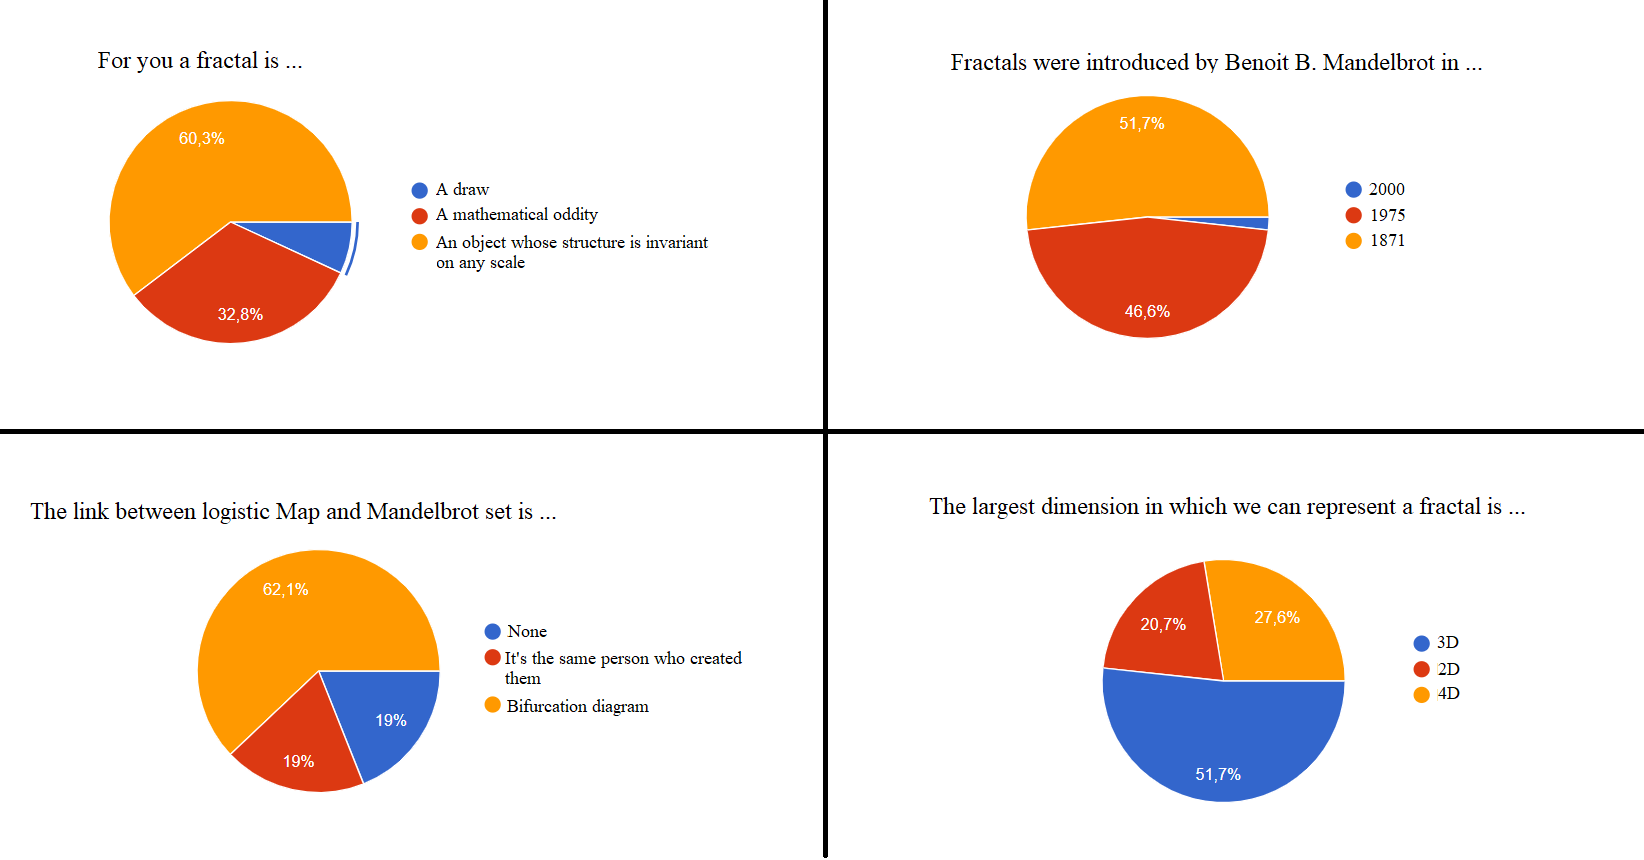
\includegraphics[width=12cm]{sondage.png}
   \end{center}
    \end{figure}
\end{frame}


\begin{frame}
\frametitle{Logistic Map}
\setbeamertemplate{blocks}[rounded][shadow=false] 
\begin{columns}[t]
  \begin{column}{5cm}
  \begin{block}{Definition of Logistic map}
 Logistic map is defined  by the following recurrence :
$$x_{n +1} =rx_n(1 - x_n)$$ 
where :
\begin{itemize}
    \item r is the growth ratio and is defined and $r \in [0,4]$
    \item $x_0 \in [0,1]$
\end{itemize}
  \end{block} 
  \end{column}
  
  \begin{column}{5cm}
  \begin{block}{Behaviour of logistic map}
The behaviour of this map is controlled by r. Indeed, when :
\begin{itemize}
    \item $r \in [0,1]$ the population die ;
    \item  $r \in ]1,3[$ the population approach the value $\frac{r-1}{r}$ ;
    \item  $r \in [3, 3.56995[$ the population oscillate between two values ;
    \item $r \geq 3.56995$ the population be chaotic.
\end{itemize}
  \end{block}   
  \end{column}
 \end{columns}

\end{frame}

\begin{frame}{Bifurcation Diagram}
    \begin{figure}[!h]
    \begin{center}
   \caption{\label{étiquette} Bifurcation Diagram}
   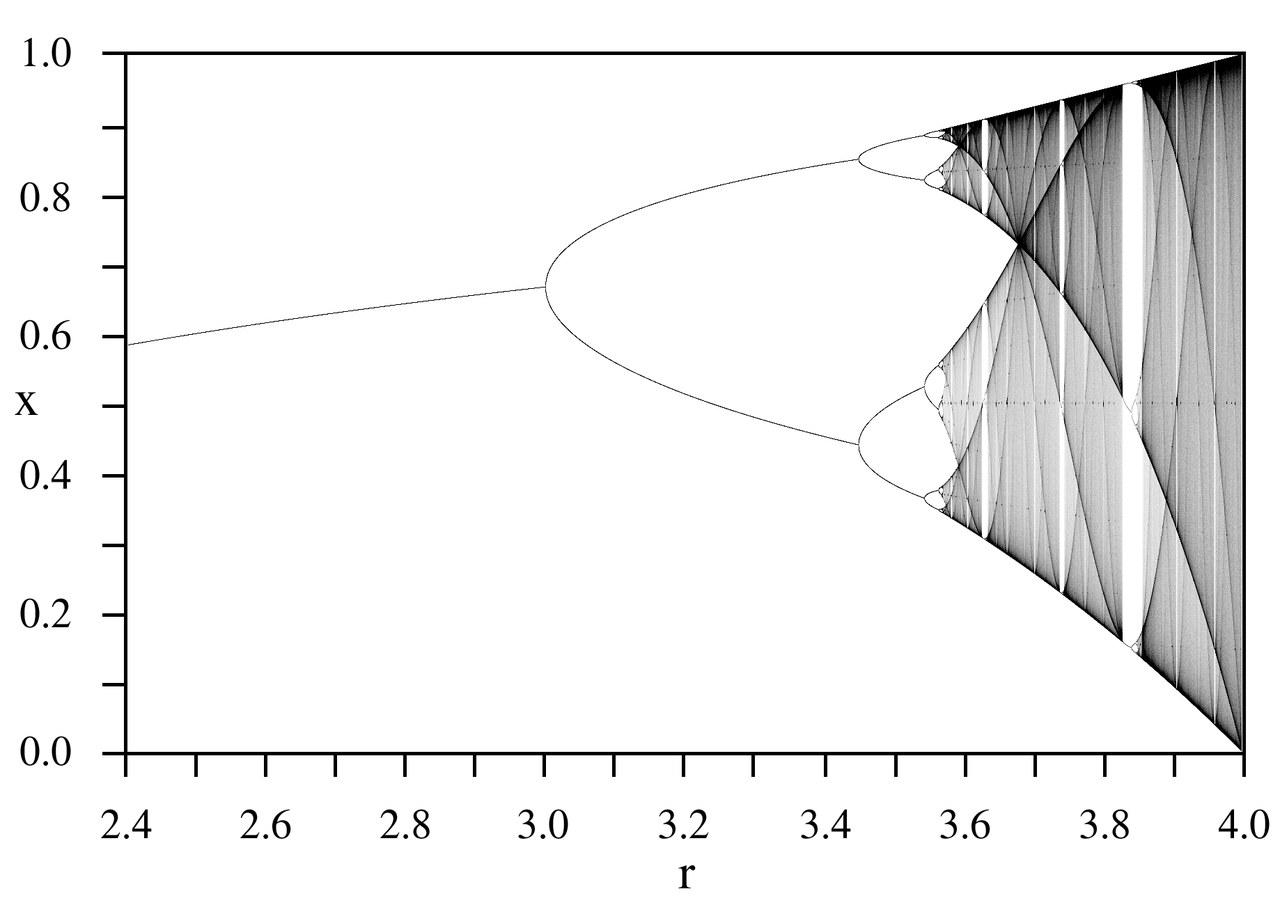
\includegraphics[width=9cm]{bifurcation.png}
   \end{center}
    \end{figure}
\end{frame}


\begin{frame}{Mandelbrot 2D}
\section{Mandelbrot 2D}
  The Mandelbrot set is a fractal set defined as the assembly of points c in the complex plan for which the sequence of complex number defined by :
	\begin{center}
	\begin{cases}
	z_0=0\\
	z_{n+1}=z_n^2+c
	\end{cases}
    \end{center}
	is bounded.  
	\begin{figure}[!h]
    \begin{center}
   \caption{\label{étiquette} Mandelbrot set}
   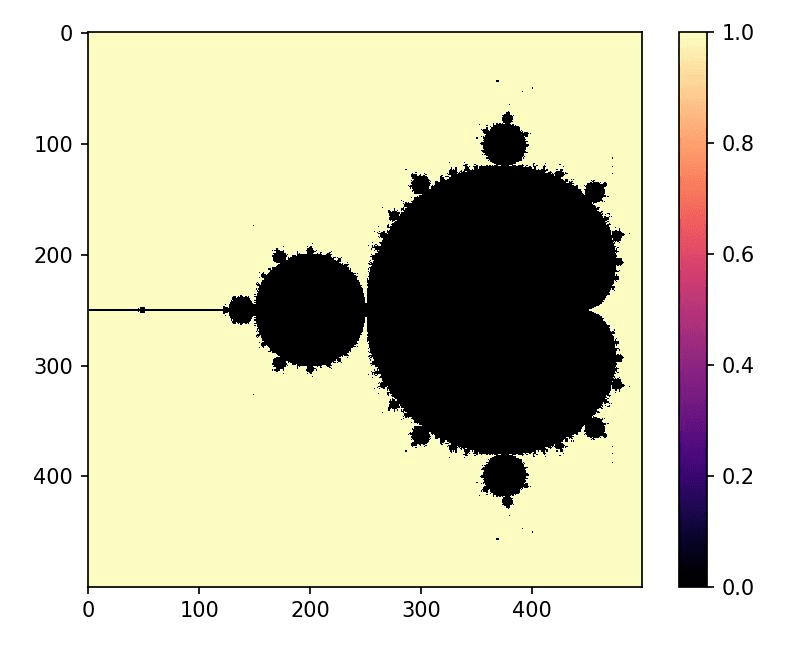
\includegraphics[width=5cm]{Mandelbrotset.png}
   \end{center}
    \end{figure}
\end{frame}

\begin{frame}{A fractal set}
	The previous picture represents the set as we see it most of the time, but changing the arguments in the function can make it a little different. We can already see it, but the set is a fractal: we can see a dozen of mini-Mandelbrot surrounding the big one, but zooming on the set makes it more obvious. Here is a picture obtained by zooming on the upper part of the picture :
    \begin{figure}[!h]
    \begin{center}
   \caption{\label{étiquette} Mini-Mandelbrots}
   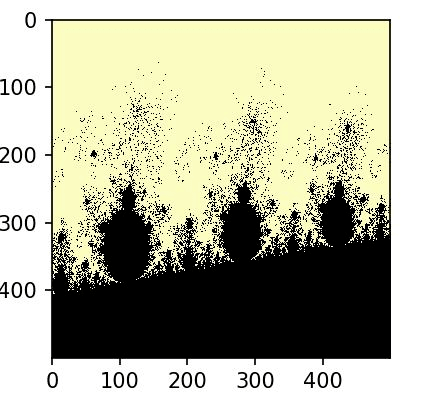
\includegraphics[width=4cm]{Mandelbrot_zoom.png}
   \end{center}
    \end{figure}
\end{frame}

\begin{frame}{Visualization of some characteristic plots}
    Zooming on the set does not only shows mini-Mandelbrots, it also shows some characteristic patterns as the "Triple spiral valleys" or the "Elephant valleys" : 
    \begin{figure}[!h]
    \begin{center}
   \caption{\label{étiquette} Triple spiral valley}
   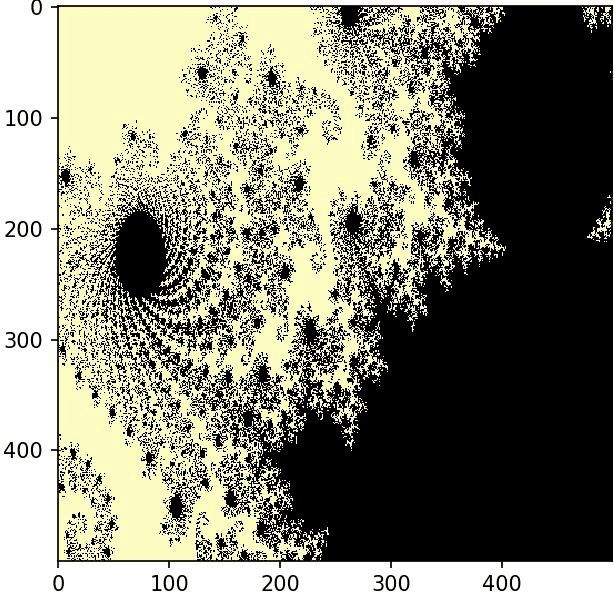
\includegraphics[width=5cm]{Triple_spiral_valley.png}
   \end{center}
    \end{figure}
\end{frame}

\begin{frame}{Visualization of some characteristic plots}
	\begin{figure}[!h]
    \begin{center}
   \caption{\label{étiquette} Elephant valley}
   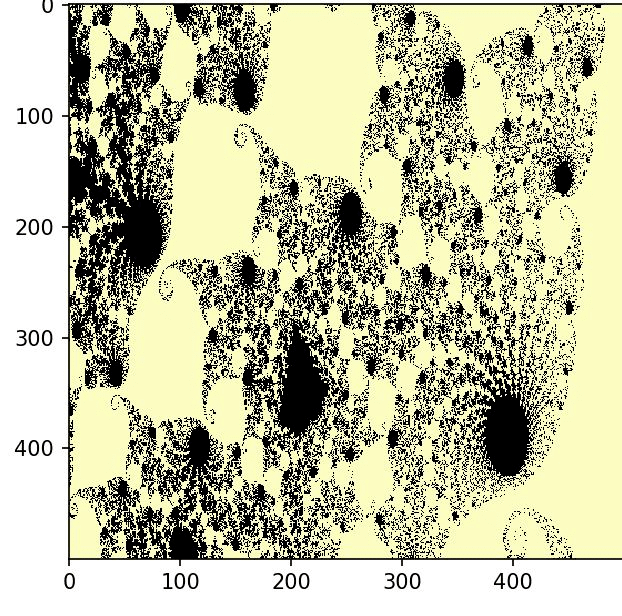
\includegraphics[width=5cm]{Elephant_valley.png}
   \end{center}
    \end{figure}
\end{frame}

\begin{frame}{Mandelbrot 3D}
\section{Mandelbrot 3D}
    As stated before, the Mandelbrot set is defined by this equation : $$z_{n+1}=z_n^2+c$$ for each c point in the complex plan. 
    
    By iterating this same equation hundreds times and plotting the values it takes on the z-axis, we can visualize the Mandelbrot set in 3D.  
    \begin{figure}[!h]
    \begin{center}
   \caption{\label{étiquette} Mandelbrot set in 3D}
   
\includegraphics[width=5cm]{Mandelbrot 3D view 0.png}
   \end{center}
    \end{figure}
\end{frame}

\begin{frame}{Rotation of the 3D Mandelbrot set}
    As far we know that the Bifurcation diagram is a fractal and the Mandelbrot set also represents a fractal.    
    
    What interest us is the connection between these two fractals.
      
    By looking at the 3D Mandelbrot from the side, we can actually see that the Bifurcation diagram is part of the Mandelbrot set.
    \begin{figure}[!h]
    \begin{center}
   \caption{\label{étiquette} Bifurcation diagram in the Mandelbrot set}
   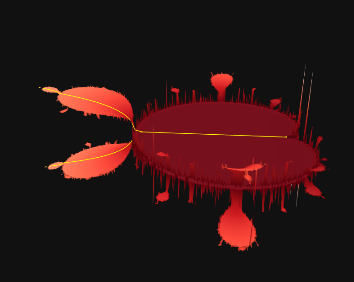
\includegraphics[width=5cm]{Mandelbrot 3D side view 0.png}
   \end{center}
    \end{figure}
\end{frame}

\begin{frame}{Conclusion}
\section{Conclusion}
    Through this project we were able to modelize some remarkable mathematical phenomena and have a better undestanding of them.
    \vspace{7}
    \newline
    First, we observed how the final state of a population was controlled by its growth ratio and how chaotic behaviour could appear starting from a simple equation.
    \vspace{7}
    \newline
    Then, we were introduced to the Mandelbrot set.
    
    Seeing how it was defined and looking into some of its many famous characteristic patterns allowed us to better grasp the concept of fractal.  
    \vspace{7}
    \newline
    Finally, by looking at the Mandelbrot set in 3D, we could highlight how the fractal was related to the Bifurcation diagram thus showing the link with mathematical results and natural phenomena.
\end{frame}



\end{document}